\documentclass[11pt, compress, aspectratio=1610]{beamer}

\usetheme{pl}

\usepackage{longtable}
\usepackage{booktabs}
\usepackage{minted}
\usepackage{listings}
\usepackage{color}
\usepackage{fancyvrb}
\newcommand{\VerbBar}{|}
\newcommand{\VERB}{\Verb[commandchars=\\\{\}]}
\DefineVerbatimEnvironment{Highlighting}{Verbatim}{commandchars=\\\{\},fontsize=\small}
% Add ',fontsize=\small' for more characters per line
\usepackage[framemethod=tikz]{mdframed}
\definecolor{shadecolor}{HTML}{EEEEEE}
\mdfsetup{
  backgroundcolor=shadecolor,
  linecolor=shadecolor,
  innerleftmargin=5pt,
  innerrightmargin=5pt,
  leftmargin=-5pt,
  rightmargin=-5pt,
  roundcorner=3pt
}
\newenvironment{Shaded}{\begin{mdframed}}{\end{mdframed}}
\newcommand{\KeywordTok}[1]{\textcolor[rgb]{0.26,0.66,0.93}{\textbf{{#1}}}}
\newcommand{\DataTypeTok}[1]{\textcolor[rgb]{0.74,0.68,0.62}{\underline{{#1}}}}
\newcommand{\DecValTok}[1]{\textcolor[HTML]{558B2F}{{#1}}}
\newcommand{\BaseNTok}[1]{\textcolor[HTML]{558B2F}{{#1}}}
\newcommand{\FloatTok}[1]{\textcolor[HTML]{558B2F}{{#1}}}
\newcommand{\ConstantTok}[1]{\textcolor[rgb]{0.74,0.68,0.62}{{#1}}}
\newcommand{\CharTok}[1]{\textcolor[HTML]{7E57C2}{{#1}}}
\newcommand{\SpecialCharTok}[1]{\textcolor[HTML]{7E57C2}{{#1}}}
\newcommand{\StringTok}[1]{\textcolor[HTML]{7E57C2}{{#1}}}
\newcommand{\VerbatimStringTok}[1]{\textcolor[HTML]{7E57C2}{{#1}}}
\newcommand{\SpecialStringTok}[1]{\textcolor[HTML]{7E57C2}{{#1}}}
\newcommand{\ImportTok}[1]{\textcolor[rgb]{0.74,0.68,0.62}{{#1}}}
\newcommand{\CommentTok}[1]{\textcolor[HTML]{546E7A}{\textit{{#1}}}}
\newcommand{\DocumentationTok}[1]{\textcolor[HTML]{BCAAA4}{\textit{{#1}}}}
\newcommand{\AnnotationTok}[1]{\textcolor[HTML]{BCAAA4}{\textbf{\textit{{#1}}}}}
\newcommand{\CommentVarTok}[1]{\textcolor[rgb]{0.74,0.68,0.62}{{#1}}}
\newcommand{\OtherTok}[1]{\textcolor[rgb]{0.74,0.68,0.62}{{#1}}}
\newcommand{\FunctionTok}[1]{\textcolor[HTML]{26A69A}{\textbf{{#1}}}}
\newcommand{\VariableTok}[1]{\textcolor[rgb]{0.74,0.68,0.62}{{#1}}}
\newcommand{\ControlFlowTok}[1]{\textcolor[rgb]{0.26,0.66,0.93}{\textbf{{#1}}}}
\newcommand{\OperatorTok}[1]{\textcolor[rgb]{0.74,0.68,0.62}{{#1}}}
\newcommand{\BuiltInTok}[1]{\textcolor[HTML]{42A5F5}{{#1}}}
\newcommand{\ExtensionTok}[1]{\textcolor[rgb]{0.74,0.68,0.62}{{#1}}}
\newcommand{\PreprocessorTok}[1]{\textcolor[rgb]{0.74,0.68,0.62}{\textbf{{#1}}}}
\newcommand{\AttributeTok}[1]{\textcolor[rgb]{0.74,0.68,0.62}{{#1}}}
\newcommand{\RegionMarkerTok}[1]{\textcolor[rgb]{0.74,0.68,0.62}{{#1}}}
\newcommand{\InformationTok}[1]{\textcolor[rgb]{0.00,0.40,1.00}{\textbf{\textit{{#1}}}}}
\newcommand{\WarningTok}[1]{\textcolor[HTML]{FF6E40}{\textbf{{#1}}}}
\newcommand{\AlertTok}[1]{\textcolor[HTML]{FF3D00}{{#1}}}
\newcommand{\ErrorTok}[1]{\textcolor[HTML]{DD2C00}{\textbf{{#1}}}}
\newcommand{\NormalTok}[1]{\textcolor[HTML]{212121}{{#1}}}

\providecommand{\tightlist}{%
  \setlength{\itemsep}{0pt}\setlength{\parskip}{0pt}}

\let\OldTexttt\texttt
\renewcommand{\texttt}[1]{\OldTexttt{\color{plTT}#1}}

\makeatletter
\def\maxwidth{\ifdim\Gin@nat@width>\linewidth\linewidth\else\Gin@nat@width\fi}
\makeatother

\usepgfplotslibrary{dateplot}

\newcommand{\begincols}{\begin{columns}}
\newcommand{\stopcols}{\end{columns}}
\newcommand{\roundpicture}[2]{%
\tikz\node[circle,
          text=white,
          minimum width=4cm,
          minimum height=4cm,
          path picture={
              \node at (path picture bounding box.center){
                  \includegraphics[width=4cm]{#1}
              };
          }]{#2};
}
\newcommand{\plain}[1]{%
\begin{picture}(0,0)
  \put(-28.5,-175){%
      \pgfuseimage{titlebackground}
  }
  \put(0,-145){%
      \begin{minipage}[b][4.5cm][t]{0.5\textwidth}
          \color{white}\huge
              #1
      \end{minipage}
  }
\end{picture}
}

\title{Quantifying the limits to population forecasts}
\subtitle{An example using the Yellowstone bison population}
\date{\today}
\author{Andrew Tredennick}
\institute{Utah State University}

\begin{document}

\maketitle

\begin{frame}{%
\protect\hypertarget{main-goals}{%
Main goals}}

\begin{enumerate}
[1.]
\tightlist
\item
  Fit Bayesian state-space model for bison population dynamics
  \alert{with} an environmental covariate
\item
  Compare out-of-sample forecasts with and without known environmental
  conditions
\item
  Partition forecast uncertainty into components
\end{enumerate}

\end{frame}

\hypertarget{the-data}{%
\section{The data}\label{the-data}}

\begin{frame}{%
\protect\hypertarget{time-series-of-bison-counts-1970---2017}{%
Time series of bison counts (1970 - 2017)}}

\begin{description}
\tightlist
\item[Response]
Bison counts
\item[Covariate]
Accumulated snow water equilivalent (West Yellowston SNOTEL)
\end{description}

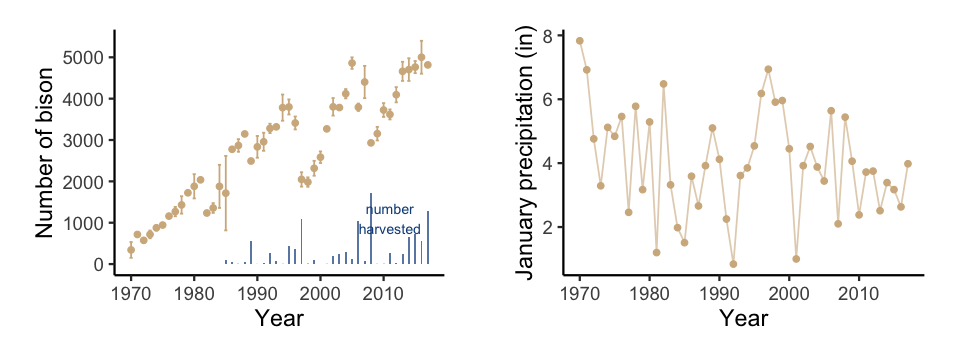
\includegraphics[width=\textwidth]{../figures/bison_data_plots.png}

\begin{center}
\textcolor{blue}{training data} $\cdot$ \textcolor{orange}{validation data}
\end{center}

\end{frame}

\hypertarget{the-model}{%
\section{The model}\label{the-model}}

\begin{frame}{%
\protect\hypertarget{gompertz-population-growth}{%
Gompertz population growth}}

\[
\text{log}(z_{(t)}) \sim \text{Normal}\left( \text{log}(z_{(t-1)}) + r + b_0 \text{log}(z_{(t-1)}) + b_1 x_{(t)}, \sigma^2_\text{p} \right)
\]

\begin{description}
\tightlist
\item[\(z_t\)]
\alert{latent} population abundance in year \emph{t}
\item[\(r\)]
per capita growth rate
\item[\(b_0\)]
density dependence
\item[\(b_1\)]
effect of snow water equivalent
\item[\(x_t\)]
accumulated snow water equivalent in year \emph{t}
\item[\(\sigma^2_\text{p}\)]
process variance
\end{description}

\end{frame}

\begin{frame}{%
\protect\hypertarget{likelihood-and-fully-specified-model}{%
Likelihood and fully specified model}}

Likelihood

\[
 y_{(t)} \sim \text{NB} \left(  z_{(t)} , \kappa \right)
 \]

Full model

\[
 \left[ \boldsymbol{\theta}_\text{p}, \kappa, z_{(t)}, z_{(t-1)} | y_{(t)}, x_{(t)} \right ] \propto \prod_{t=2}^{58} \underbrace{\left[ z_{(t)} | \boldsymbol{\theta}_\text{p}, z_{(t-1)}, x_{(t)} \right]}_{\text{process}} \prod_{t=1}^{48} \underbrace{\left[ y_{(t)} | \kappa, z_{(t)} \right]}_{\text{data}} \underbrace{\left[ \boldsymbol{\theta}_\text{p}, \kappa, z_{(t=1)}\right]}_{\text{parameters}}
 \]

Includes a strong prior on \(r\) based on Hobbs et al.~2015:
\(r \sim \text{Normal}(0.1, 0.02)\)

\end{frame}

\hypertarget{results}{%
\section{Results}\label{results}}

\begin{frame}{%
\protect\hypertarget{posterior-distributions-of-parameters}{%
Posterior distributions of parameters}}

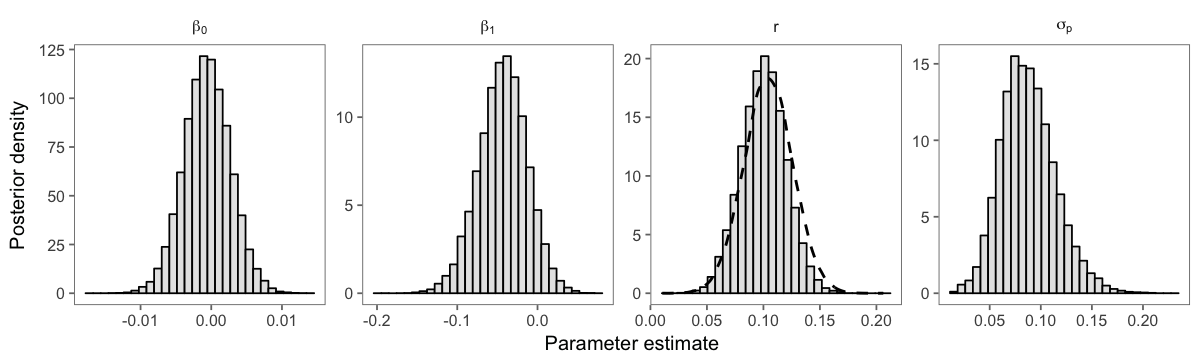
\includegraphics[width=\textwidth]{../figures/bison_post_params.png}

\alert{Note}: posterior distrbution of \(r\) totally informed by prior.

\end{frame}

\begin{frame}{%
\protect\hypertarget{posterior-predictions-forecasts-and-forecast-partition}{%
Posterior predictions, forecasts, and forecast partition}}

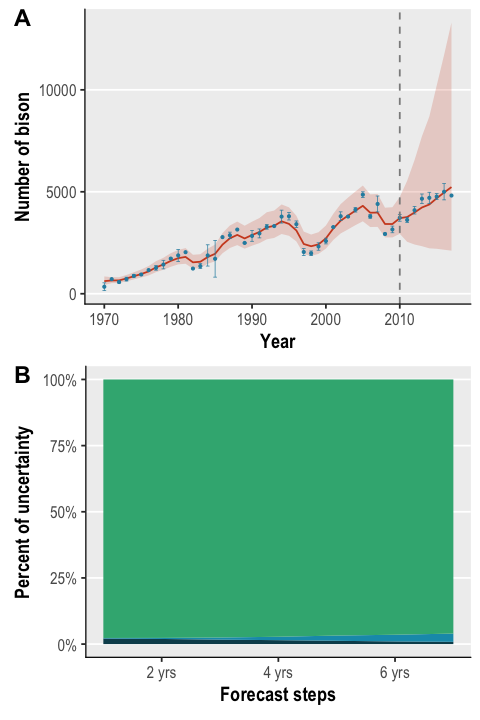
\includegraphics[height=\textheight]{../figures/bison_combined.png}

\end{frame}

\hypertarget{take-home-messages}{%
\section{Take home messages}\label{take-home-messages}}

\begin{frame}{%
\protect\hypertarget{take-home}{%
Take home}}

\begin{enumerate}
[1.]
\tightlist
\item
  Snow water equivalent effect is weak – right covariate?
\item
  Forecast uncertainty is large.
\item
  Forecast unceratinty dominated by (simulated) uncertainty of snow
  water equivalent
\end{enumerate}

\end{frame}

\begin{frame}[plain]
  \begin{picture}(0,0)
    \put(-28.5,-175){%
      \pgfuseimage{titlebackground}
    }
  \end{picture}
\end{frame}

\end{document}
